\documentclass[12pt]{exam}
\usepackage{amsthm}
\usepackage{bm}
\usepackage{libertine}
\usepackage[utf8]{inputenc}
\usepackage[margin=0.5in]{geometry}
\usepackage{amsmath,amssymb}
\usepackage{multicol}
\usepackage[shortlabels]{enumitem}
\usepackage{siunitx}
\usepackage{physics}
\usepackage{booktabs}
\usepackage{graphicx}
\usepackage{pgfplots}
\usepackage{listings}
\usepackage{tikz}
\usepackage{tikz-3dplot}
\usetikzlibrary{arrows.meta,decorations.markings}

\bmdefine{\ii}{i}
\bmdefine{\jj}{j}
\bmdefine{\kk}{k}
\newcommand{\te}{\theta}
\newcommand{\cC}{\mathcal{C}}
\newcommand{\word}[1]{\quad\text{#1}\quad}

\pgfplotsset{width=10cm,compat=1.9}
\usepgfplotslibrary{external}
\tikzexternalize
% Compile the small black-and-white solution diagram inline.
\tikzexternaldisable

\newcommand{\class}{Math 261-001}
\newcommand{\examnum}{Quiz 8 Solutions}
\newcommand{\examdate}{October 30}

\begin{document}
\pagestyle{plain}
\thispagestyle{empty}

\noindent
\textbf{\class}\\
\textbf{\examnum}, \textbf{\examdate}

\vspace{8pt}
\small
\setlength{\abovedisplayskip}{6pt}
\setlength{\belowdisplayskip}{6pt}
\setlength{\abovedisplayshortskip}{3pt}
\setlength{\belowdisplayshortskip}{6pt}
\begin{enumerate}

\item \textbf{Final answer:} $\boxed{42\pi}$.

Parametrize the graph by $\vec r(x,y)=(x,y,xy)$ over the disk
$D: x^2+y^2\le15$. Its tangent vectors and area factor are
\[
\begin{aligned}
\vec r_x&=(1,0,y),& \vec r_y&=(0,1,x),\\
\vec n = \vec r_x\times\vec r_y&=(-y,-x,1),&
\|\vec n\|&=\sqrt{1+x^2+y^2}.
\end{aligned}
\]
Convert the double integral over $D$ to polar coordinates, with bounds
\[
\left\{
\begin{aligned}
&0\le\theta\le2\pi,\\
&0\le r\le\sqrt{15}.
\end{aligned}
\right.
\]
Thus
\[
\begin{aligned}
\operatorname{Area}(S)
&=\iint_D\sqrt{1+x^2+y^2}\,dA\\
&=\int_0^{2\pi}\int_0^{\sqrt{15}}r\sqrt{1+r^2}\,dr\,d\theta\\
&=\frac{2\pi}{3}\left[(1+r^2)^{3/2}\right]_0^{\sqrt{15}}
=\frac{2\pi}{3}(64-1)=42\pi.
\end{aligned}
\]
Here the factor $r$ comes from $dA=r\,dr\,d\theta$. A direct polar
parametrization of the surface gives the same area factor:
\[
\vec f(r,\theta)=(r\cos\theta,r\sin\theta,r^2\cos\theta\sin\theta),
\qquad \|\vec f_r\times\vec f_\theta\|=r\sqrt{1+r^2}.
\]

\medskip
\item \textbf{Final answer:} $\boxed{35\pi}$.

The parametrization of the curve in question is \(\vec r(t)=(t,3t/4)\) with \(2\leq t\leq 4\). A parametrization of
the curved lampshade is
\[
\vec f(t,\theta)=\left(t\cos\theta,\frac{3t}{4},-t\sin\theta\right),
\qquad
\left\{
\begin{aligned}
&2\le t\le4,\\
&0\le\theta\le2\pi.
\end{aligned}
\right.
\]
Its tangent vectors give
\[
\begin{aligned}
\vec f_t&=\left(\cos\theta,\frac34,-\sin\theta\right),&
\vec f_\theta&=(-t\sin\theta,0,-t\cos\theta),\\
\vec n = \vec f_\theta\times\vec f_t
&=\left(\frac{3t}{4}\cos\theta,-t,-\frac{3t}{4}\sin\theta\right),&
\|\vec n\|&=\frac{5t}{4}.
\end{aligned}
\]
This order gives an outward normal.
The surface density becomes $\delta(\vec f(t,\theta))=3t/4$, so
\[
\begin{aligned}
M&=\iint_S\sigma\,dS
=\int_0^{2\pi}\int_2^4\frac{3t}{4}\frac{5t}{4}\,dt\,d\theta\\
&=\frac{15\pi}{8}\left[\frac{t^3}{3}\right]_2^4
=\frac{5\pi}{8}(64-8)=35\pi.
\end{aligned}
\]

\newpage

\item \textbf{Final answers:}
\[
\boxed{\text{(a) }\vec r_\phi\times\vec r_\theta},\qquad
\boxed{\text{(b) }\vec f_\theta\times\vec f_t},\qquad
\boxed{\text{(c) }\vec r_u\times\vec r_v}.
\]
In each diagram, the two tangent vectors and the normal $\vec n$ start
at the marked point $P$. Arrow lengths are rescaled for readability.

\begin{enumerate}[label=(\alph*)]
\item For the ellipsoid,
\[
\vec r_\phi\times\vec r_\theta
=\left(3\sin^2\phi\cos\theta,
2\sin^2\phi\sin\theta,6\sin\phi\cos\phi\right).
\]
\noindent\begin{minipage}[c]{0.54\linewidth}
\raggedright
Let $f(x,y,z)=x^2/4+y^2/9+z^2$. Then the normal vector can be seen to be
\[
\vec r_\phi\times\vec r_\theta
=3\sin\phi\,\nabla f(\vec r(\theta,\phi)).
\]
Since $0<\phi<\pi$, the sine is positive, and $\nabla f$ points
outward from the ellipsoid, which is the surface $f=1$.\par
\smallskip
At $(\theta,\phi)=(0,\pi/2)$, the marked point is $P=(2,0,0)$, and
\[
\begin{aligned}
\vec r_\phi&=(0,0,-1),\\
\vec r_\theta&=(0,3,0),\\
\vec n&=(3,0,0).
\end{aligned}
\]
The normal points along the positive $x$-axis, outward from the ellipsoid.
\end{minipage}\hfill
\begin{minipage}[c]{0.43\linewidth}
\centering
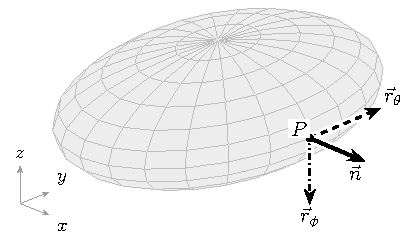
\includegraphics[width=\linewidth,height=4.8cm,keepaspectratio]{figures/q8-ellipsoid-frame.pdf}
\end{minipage}

\medskip
\item For the cylinder around the $y$-axis,
\[
\vec f_\theta=(-\sin\theta,0,-\cos\theta),\qquad
\vec f_t=(0,1,0),\qquad
\vec f_\theta\times\vec f_t=(\cos\theta,0,-\sin\theta).
\]
\noindent\begin{minipage}[c]{0.54\linewidth}
\raggedright
This is exactly the radial vector from the $y$-axis to the surface point.
At $(t,\theta)=(1,0)$, the marked point is $P=(1,1,0)$, and
\[
\begin{aligned}
\vec f_\theta&=(0,0,-1),\\
\vec f_t&=(0,1,0),\\
\vec n&=(1,0,0).
\end{aligned}
\]
The normal points away from the axis; both tangent vectors lie in the
tangent plane to the curved wall.
\end{minipage}\hfill
\begin{minipage}[c]{0.43\linewidth}
\centering
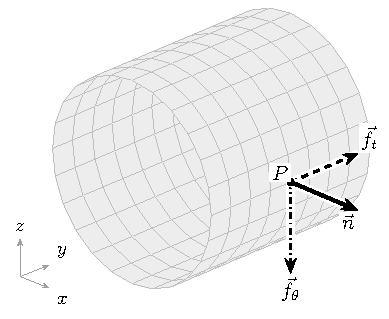
\includegraphics[width=\linewidth,height=4.8cm,keepaspectratio]{figures/q8-cylinder-frame.pdf}
\end{minipage}

\medskip
\item For the graph $\vec r(u,v)=(u,v,u^2+v^2)$,
\[
\vec r_u=(1,0,2u),\qquad \vec r_v=(0,1,2v),\qquad
\vec r_u\times\vec r_v=(-2u,-2v,1).
\]
\noindent\begin{minipage}[c]{0.54\linewidth}
\raggedright
Its positive third component makes the normal upward.
At $(u,v)=(-1/2,-1/2)$, the marked point is
$P=(-1/2,-1/2,1/2)$, and
\[
\begin{aligned}
\vec r_u&=(1,0,-1),\\
\vec r_v&=(0,1,-1),\\
\vec n&=(1,1,1).
\end{aligned}
\]
The diagram shows a bounded patch of the graph. The upward normal is
perpendicular to the surface, not necessarily vertical.
\end{minipage}\hfill
\begin{minipage}[c]{0.43\linewidth}
\centering
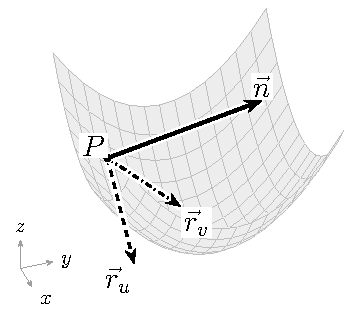
\includegraphics[width=\linewidth,height=4.8cm,keepaspectratio]{figures/q8-paraboloid-frame.pdf}
\end{minipage}
\end{enumerate}

\newpage
\item \textbf{Final answers:}
\[
\boxed{\text{(a) }\vec b},\qquad
\boxed{\text{(b) }s+t\le1}.
\]
Since $\vec{PQ}=Q-P=(2,0,0)$ and $\vec{PR}=R-P=(0,3,3)$,
the affine parametrization is
\[
\vec a(s,t)=s\vec{PQ}+t\vec{PR}+P=(2s,3t,1+3t).
\]
With the whole unit square as its domain, its four corners map to
$P$, $Q$, $R$, and $Q+R-P=(2,3,4)$. Therefore its image is a
parallelogram, not just the given triangle.

For the ruled parametrization,
\[
\vec b(s,t)=t\bigl((s\vec{PQ}+P)-R\bigr)+R
=(2st,3-3t,4-3t),
\]
the point $s\vec{PQ}+P=(1-s)P+sQ$ runs along the edge $PQ$.
As $t$ varies from $0$ to $1$, the ruling joins $R$ to that point.
These rulings cover exactly the given triangle. The collapsed edge
$t=0$ maps to the vertex $R$.

\medskip
\noindent\begin{minipage}[c]{0.63\linewidth}
To correct the domain of $\vec a$, we add $s+t\le1$, giving the bounds
\[
\left\{
\begin{aligned}
&0\le s\le1,\\
&0\le t\le1-s.
\end{aligned}
\right.
\]
The shaded parameter triangle maps to the given triangle; the remaining half of
the square is the extra part of the parallelogram.
\end{minipage}\hfill
\begin{minipage}[c]{0.33\linewidth}
\centering
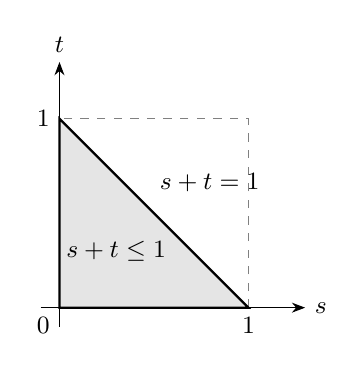
\begin{tikzpicture}[x=2.4cm,y=2.4cm,>=Stealth,
every node/.style={font=\small}]
\fill[gray!20] (0,0)--(1,0)--(0,1)--cycle;
\draw[gray,dashed] (1,0)--(1,1)--(0,1);
\draw[thick] (0,0)--(1,0)--(0,1)--cycle;
\draw[->] (-0.1,0)--(1.3,0) node[right] {$s$};
\draw[->] (0,-0.1)--(0,1.3) node[above] {$t$};
\node[below left] at (0,0) {$0$};
\node[below] at (1,0) {$1$};
\node[left] at (0,1) {$1$};
\node[above right] at (0.48,0.56) {$s+t=1$};
\node at (0.3,0.3) {$s+t\le1$};
\end{tikzpicture}
\end{minipage}

\end{enumerate}
\end{document}
